\begin{enumerate}[label=\thesubsection.\arabic*,ref=\thesubsection.\theenumi]
\item Construct a triangle $ABC$ in which $BC=7cm, \angle{B}=75\degree$ and $AB + AC = 13 cm$.
\label{chapters/9/11/2/1}
	\\
	\solution 
		From 
		\eqref{eq:9/11/2/1}
		and 
		\eqref{eq:9/11/2/1-final},
		we obtain
		\figref{fig:9/11/2/1}.
		\iffalse
		See
\begin{lstlisting}
	codes/triangle/const-aBsum.py
\end{lstlisting}
\fi
	\begin{figure}[H]
		\centering
 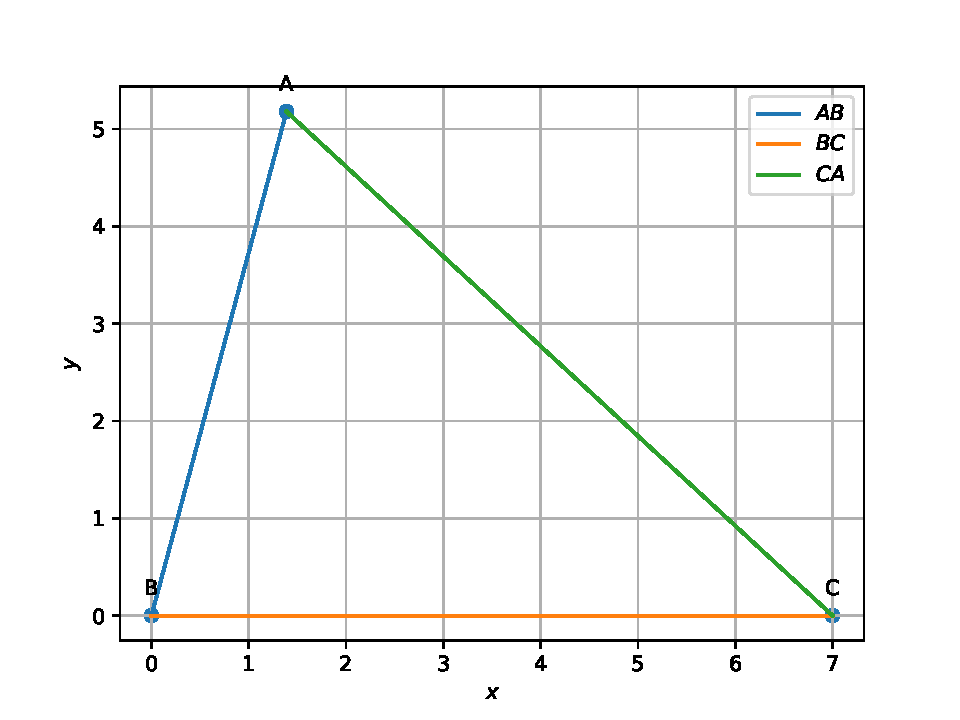
\includegraphics[width=0.75\columnwidth]{chapters/9/11/2/1/figs/vector.pdf}
		\caption{}
		\label{fig:9/11/2/1}
  	\end{figure}
	

%
\item Construct a triangle $ABC$ in which $BC=8cm, \angle{B}=45\degree$ and $AB - AC = 3.5 cm$.
\label{chapters/9/11/2/2}
\\
\solution
See \figref{fig:Fig1}.
\begin{figure}[H]
 \begin{center}
	 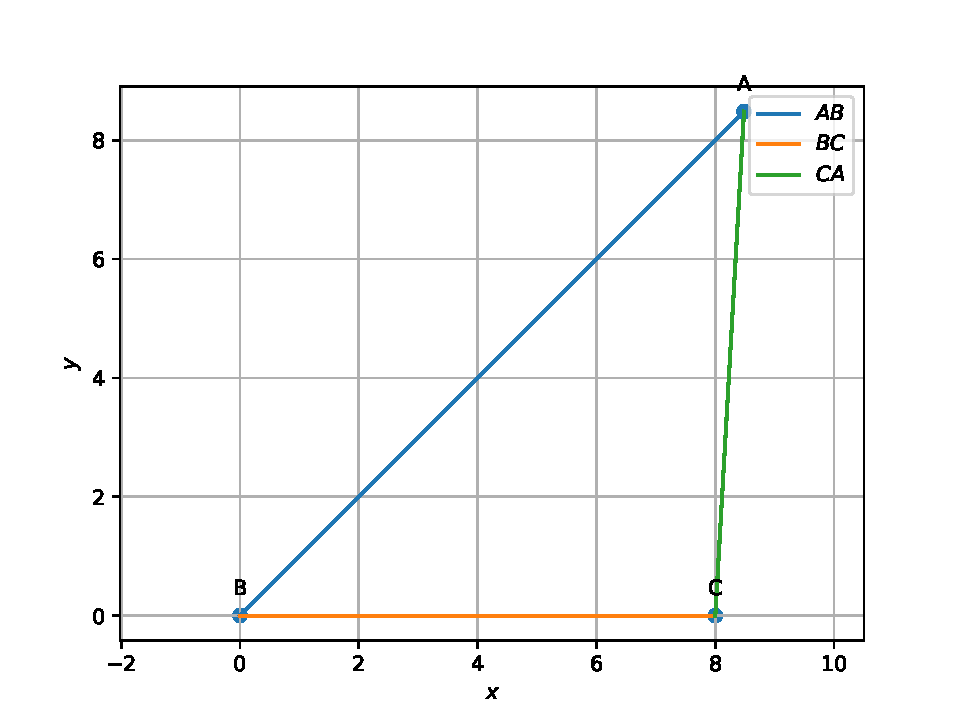
\includegraphics[width=0.75\columnwidth]{chapters/9/11/2/2/figs/vector.pdf}
 \end{center}
 \caption{}
 \label{fig:Fig1}
\end{figure}

%
\item Construct a triangle $ABC$ in which $BC=6cm, \angle{B}=60\degree$ and $AC - AB = 2cm$.
\label{chapters/9/11/2/3}
\\
\solution 
\iffalse
\documentclass[10pt,a4paper]{article}
\usepackage{amsmath}
\usepackage{amsfonts}
\usepackage{amssymb}
\usepackage{graphicx}
\usepackage{multicol}
\usepackage{tabularx}
\usepackage{tikz}
\usetikzlibrary{arrows,shapes,automata,petri,positioning,calc}
\usepackage{hyperref}
\usepackage{tikz}
\usepackage{gensymb}
\usepackage{polynom}
\usetikzlibrary{matrix,calc}
\makeatletter
\newcommand\xleftrightarrow[2][]{%
  \ext@arrow 9999{\longleftrightarrowfill@}{#1}{#2}}
\newcommand\longleftrightarrowfill@{%
  \arrowfill@\leftarrow\relbar\rightarrow}
\makeatother
\usepackage[margin=0.5in]{geometry}
\newcommand{\myvec}[1]{\ensuremath{\begin{pmatrix}#1\end{pmatrix}}}
\let\vec\mathbf
\newenvironment{Figure}
  {\par\medskip\noindent\minipage{\linewidth}}
  {\endminipage\par\medskip}
\begin{document}
%--------------------logo figure-------------------------%
\begin{figure*}[!tbp]
 \centering
  \begin{minipage}[b]{0.4\textwidth}
  
\includegraphics[scale=.25]{iitlogo.png} 
  \end{minipage}
\end{figure*}
%--------------------name & rollno-----------------------
\raggedright \textbf{Name}:\hspace{1mm} Ganga Gopinath\hspace{3cm} \Large \textbf{Matrix Assignment}\hspace{2.5cm} % 
\normalsize \textbf{Roll No.} :\hspace{1mm} FWC22050\vspace{1cm}
\begin{multicols}{2}
\section{Problem statement:}
\fi
	\begin{figure}[!h]
		\centering
 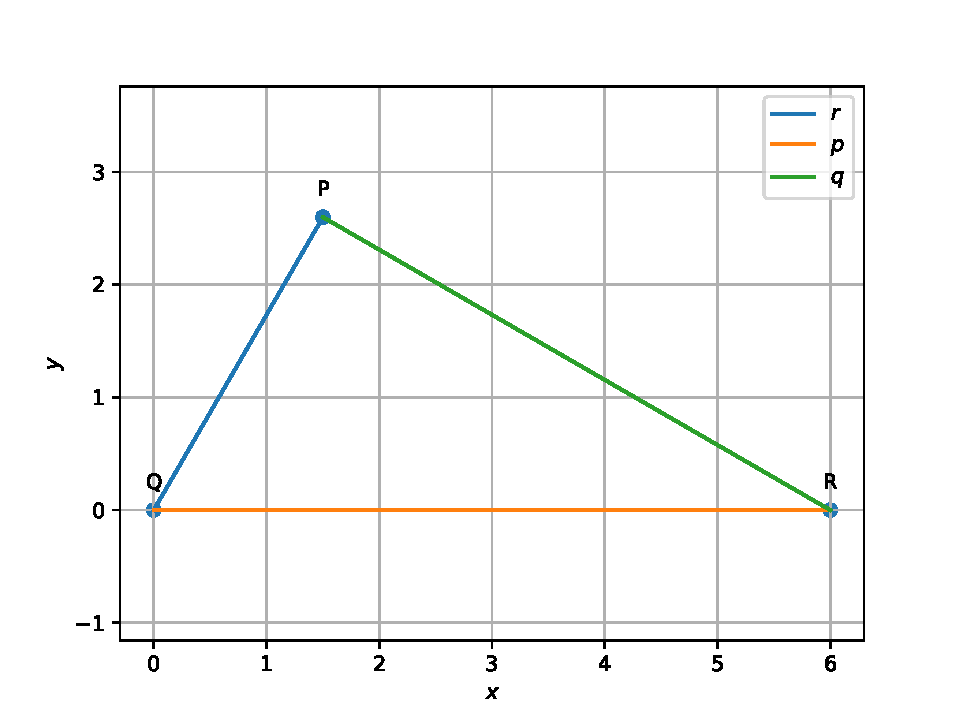
\includegraphics[width=\columnwidth]{chapters/9/11/2/3/figs/line1.pdf}
		\caption{}
		\label{fig:9/11/2/3}
  	\end{figure}
	\solution  Same as Problem 
\ref{chapters/9/11/2/1} with 
\begin{align}
\angle Q = \angle B, QR = a, PR = b, PQ = c
\end{align}
\iffalse

\textbf{Law of Cosines}
\vspace{2mm}\raggedright \\

The law of Cosines relates the length of the triangle to the cosines of one of its angles. It states that, if the length of two sides and the angle between them is known for a triangle, then we can determine the length of the third side. It is given by:
\begin{equation}
\alpha^2=\beta^2+\gamma^2-2\beta\gamma\cos\theta
\end{equation}
%-----------------------------solution---------------------------
\raggedright \textbf{SOLUTION}:\vspace{5mm}\\
\raggedright \textbf{Steps of Construction:}\vspace{2mm}\\
\textbf{Step 1:}\vspace{2mm}\\
Let P,Q and R be the vertices of the triangle  with coordinates.

Given QR length is a=6cm,
So the coordinates of vertices  Q,R and P are :\vspace{2mm}\\
\begin{center}$
{
 Q =\begin{pmatrix}
0 \\
0 
\end{pmatrix} 
\vspace{1mm}
R=\begin{pmatrix}
6 \\
0 
\end{pmatrix} 
\vspace{1mm}
P=\alpha\begin{pmatrix}
cos \theta\\
  sin \theta\\
\end{pmatrix} }
\vspace{1mm}$
\end{center}
Also given the angle is $Q=60^0$,so by finding the coordinates of the other sid
    e we can form a required triangle. \\
 \vspace{2mm}
For the input parameters in Table 1.\\
{\setlength\extrarowheight{2pt}
\begin{center}
\begin{tabular}{|c|c|c|}
	\hline
	\textbf{Symbol}&\textbf{Value}&\textbf{Description}\\
	\hline
	Q&$\begin{pmatrix}
	0\\0\\
	\end{pmatrix} $& Q Point\\
	\hline
	R&$\begin{pmatrix}
	6\\0\\
	\end{pmatrix} $& R Point\\
	\hline
	$\theta$&60$^{\circ}$&$\angle$PQR\\
	\hline
	$\lambda$ & 2 & PR-PQ\\
	\hline
	q&$\alpha$  & PR\\
	\hline
	r &$\gamma$  & PQ\\
	\hline
	p & 6 & QR\\
	\hline
\end{tabular}
%}\\
\\ {Table 1}\\
\end{center}
\vspace{3mm} 
Given that,
\begin{equation}
	\alpha-\gamma=2
\end{equation}
By using the Cosine formula in  $\Delta$PQR \\ 
\begin{equation}
\alpha^2=\beta^2+\gamma^2-2\beta\gamma\cos\theta 
\end{equation}
\vspace{1mm}
\begin{equation}
\alpha^2-\gamma^2=\beta^2-2\beta\gamma\cos\theta
\end{equation}
\vspace{1mm}
\begin{equation}
(\alpha+\gamma)(\alpha-\gamma)=\beta^2-2\beta\gamma\cos\theta
\end{equation}
\vspace{1mm}
\begin{equation}
(\alpha+\gamma)(\lambda)=\beta^2-2\beta\gamma\cos\theta
\end{equation}
\vspace{1mm}
\begin{equation}
\lambda\alpha +\lambda \gamma +2\beta\gamma\cos\theta=\beta^2
\end{equation}
\vspace{1mm}
\begin{equation}
\lambda \alpha +\gamma(\lambda+2\beta\cos\theta)=\beta^2
\end{equation}
\vspace{1mm}
%\begin{center}
%	$0=6^2+\gamma^2 -\alpha^2-2\times \gamma \times 6 \times cos60$\\

%\vspace{5mm}
%\end{center}
%After simplification
%\begin{equation}
%	   4\gamma+\alpha =18
%\end{equation}

\textbf{Step 2:}\vspace{2mm}\\
We know that,\\
\begin{equation}
\vec{A  X = B}
\end{equation}
Using equation (2) and (8),


\begin{equation}
  \begin{pmatrix}
1 & -1\\
\lambda & \lambda+2\beta\cos\theta
\end{pmatrix} 
\begin{pmatrix}
\alpha\\
\gamma
\end{pmatrix} 
=
\begin{pmatrix}
\lambda\\ 
 \beta^2\
\end{pmatrix}
\end{equation}\vspace{2mm}\\
 
After substituting values,
\begin{equation}
  \begin{pmatrix}
1 & -1\\
1 &4
\end{pmatrix} 
\begin{pmatrix}
\alpha\\
\gamma
\end{pmatrix} 
=
\begin{pmatrix}
2\\ 
 18\
\end{pmatrix}
\end{equation}\vspace{2mm}\\


The augmented matrix for the above matrix equation is 
\vspace{3mm}
\begin{equation}
\begin{pmatrix}
  1 & -1 & \vrule & 2\\
  1 & 4  &\vrule & 18
    \end{pmatrix}  
    \end{equation} 
    
  \begin{center}
  $ \xleftrightarrow{\text{$R_2$ $\leftarrow {R_2}-{R_1}$}} $
$\begin{pmatrix}
 1 & -1& \vrule & 2\\
 0 & 5  &\vrule & 16\
  \end{pmatrix}$
  \\
  \end{center}
  
  \begin{center}
$ \xleftrightarrow{\text{$R_2$ $\leftarrow  \frac{1}{5}{R_2}$}} $
$\begin{pmatrix}
 1 & -1 & \vrule & 2\\
  0 & 1  &\vrule & \frac{16}{5}\
  \end{pmatrix}$
  \\
  \end{center}    
  
  \begin{center}
  $ \xleftrightarrow{\text{$R_1$ $\leftarrow  {R_1}+{R_2}$}} $
$\begin{pmatrix}
  1 & 0 & \vrule & \frac{26}{5}\\
  0 & 1  &\vrule & \frac{16}{5}\
  \end{pmatrix}$
  \\
  \end{center}

  \begin{equation}
\implies X = 
   \begin{pmatrix}
   \frac {26}{5}\\ 
   \frac{16}{5}
 \end{pmatrix}
 \end{equation}
Using equation (7) we get ,
\begin{equation}
	\alpha = \frac{26}{5} \vspace{2mm}
\end{equation}
\begin{equation}
	\gamma= \frac{16}{5}\vspace{2mm}
\end{equation}
The vertices of $\Delta$ PQR are \\
\begin{equation}
P= \frac{26}{5} \begin{pmatrix}
cos 60\\
sin 60\\
\end{pmatrix} 
,Q= \begin{pmatrix}
 0\\
 0\\
 \end{pmatrix} 
,R= \begin{pmatrix}
 6\\
 0\\
\end{pmatrix} 
\end{equation} \vspace{2mm}


\textbf{Result} 
\begin{center}
	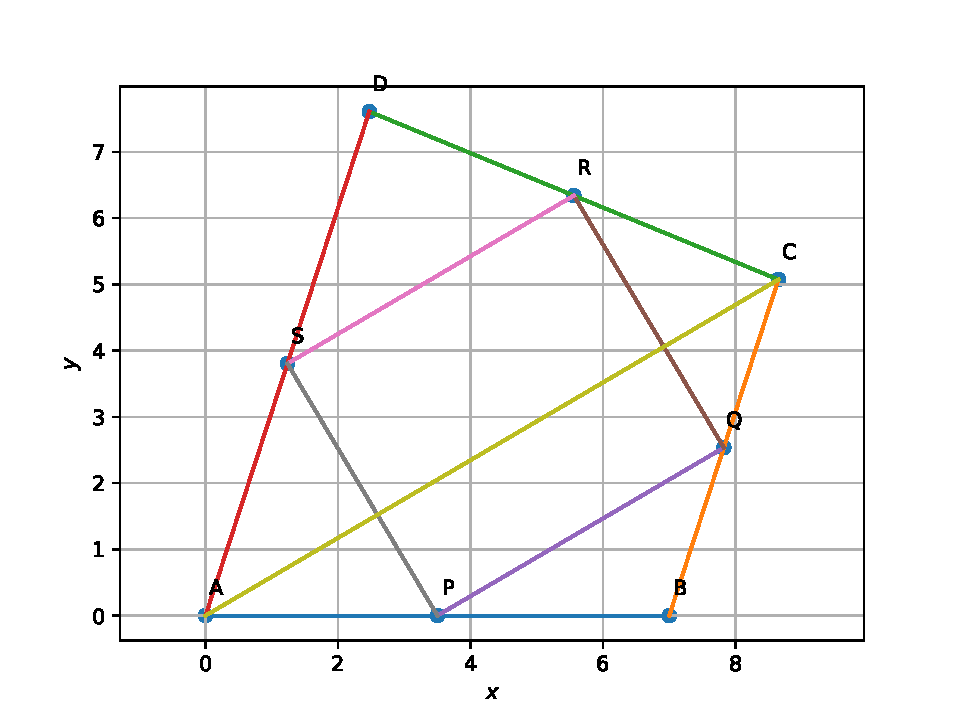
\includegraphics[width=0.4\textwidth]{line1.pdf}
\end{center}\vspace{5mm}

\vspace{4mm}  
\textbf{Implementation}
\begin{center}
\setlength{\arrayrulewidth}{0.5mm}
\setlength{\tabcolsep}{5pt}
\renewcommand{\arraystretch}{3}
    \begin{tabular}{|l|c|}
    \hline 
    \textbf{Equation no} & \textbf{Role} \\ \hline
    1 &  law of Cosines \\ 
    7 & Matrix form of Linear equation  \\
    10 & Length of r\\
    11& Length of q \\
    
    \hline
      \end{tabular}
  \end{center} \vspace{2mm} 



  \vspace{2mm} \textbf{Construction}
\begin{center}
\setlength{\arrayrulewidth}{0.5mm}
\setlength{\tabcolsep}{6pt}
\renewcommand{\arraystretch}{1.5}
    \begin{tabular}{|l|c|}
  \hline 
  \textbf{vertex} & \textbf{coordinates} \\ \hline
P & $ \begin{pmatrix} 
2.6 \\
4.5
\end{pmatrix} $ \\ \hline
   Q & $\begin{pmatrix}
0 \\
0
\end{pmatrix}$   \\\hline
   R & $\begin{pmatrix}
6 \\
0
\end{pmatrix} $\\
   \hline
    \end{tabular}
\end{center}
  
  
 
\raggedright  Download the code \\
https://github.com/Gangagopinath/ASSIGNMENT/tree/
\newline
main/assignment4
}  \end{multicols}
\end{document}
\fi

%
\item Construct a right triangle whose base is 12$cm$ and sum of its hypotenuse and other side is 18$cm$.
\label{chapters/9/11/2/5}
\\
\solution
For $a = 12, \angle B = 90\degree, b+c = 18$, we obtain 
		\figref{fig:9/11/2/5}.
	\begin{figure}[H]
		\centering
 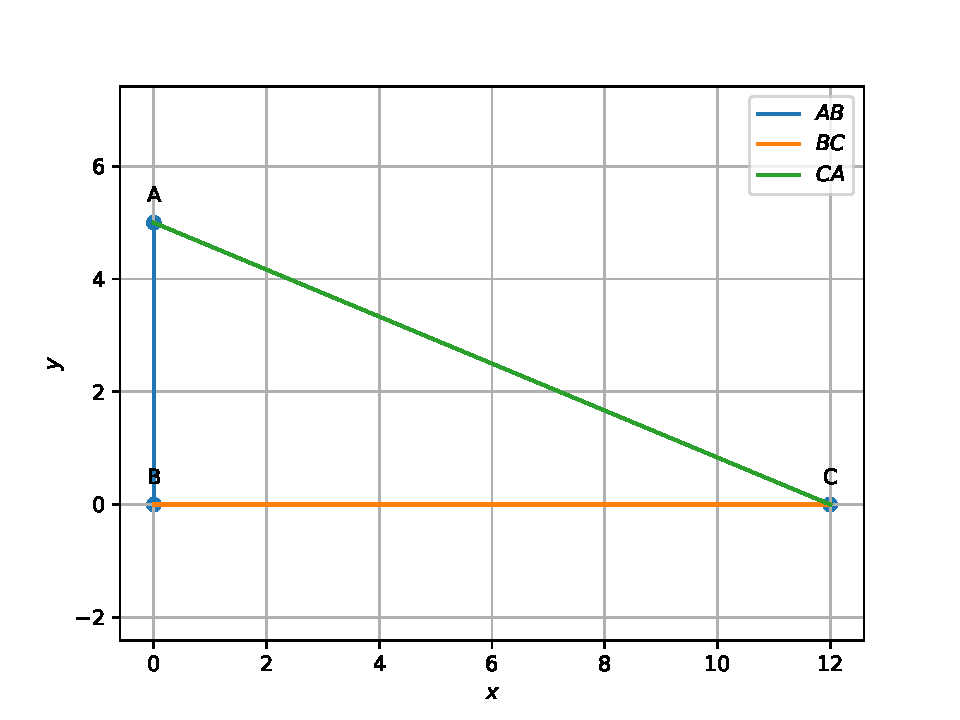
\includegraphics[width=0.75\columnwidth]{chapters/9/11/2/5/figs/vector.pdf}
		\caption{}
		\label{fig:9/11/2/5}
  	\end{figure}

%
\item Construct a triangle $ABC$ in which $\angle{B}=30\degree, \angle{C}=90\degree$ and  $AB+BC+CA=11cm$.
\label{chapters/9/11/2/4}
\\
\solution 
From 
		\eqref{eq:9/11/2/4}
		and
		\eqref{eq:9/11/2/4-final},
		\figref{fig:9/11/2/4}
		is generated.
		See
\begin{lstlisting}
	codes/triangle/const-BCsum.py
\end{lstlisting}
	\begin{figure}[!h]
		\centering
 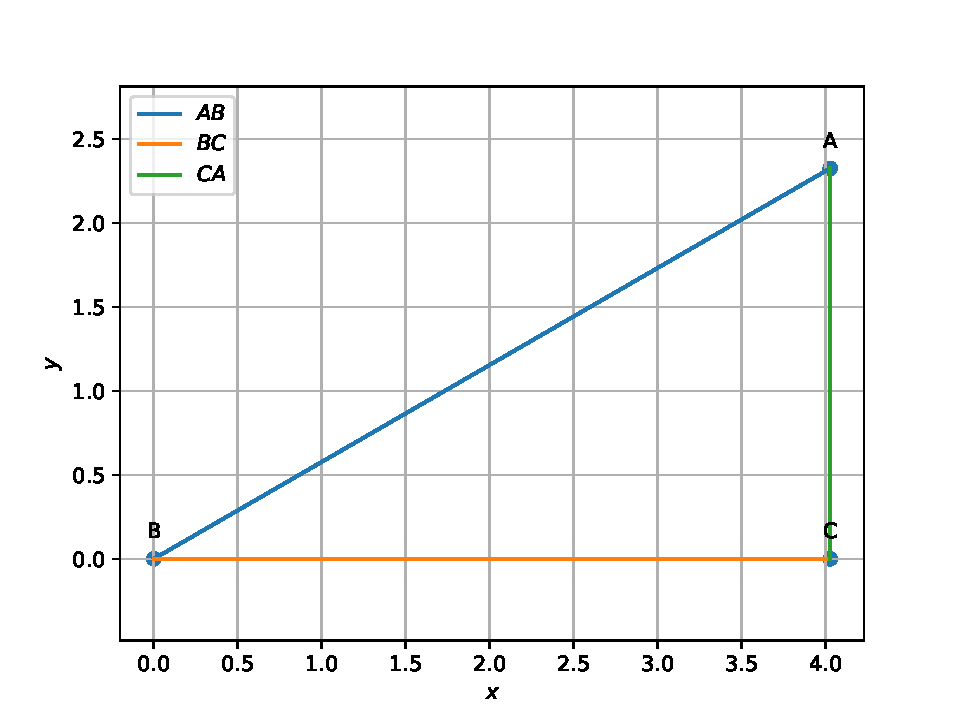
\includegraphics[width=\columnwidth]{chapters/9/11/2/4/figs/vector.pdf}
		\caption{}
		\label{fig:9/11/2/4}
  	\end{figure}

%
\item Draw a right triangle ${ABC}$ in which $BC=12 cm$, $AB=5 cm$ and $\angle{B}=90\degree$.
\item Draw an isosceles triangle ${ABC}$ in which $AB=AC=6cm$ and $BC =6cm$.
\item Draw a triangle ${ABC}$ in which $AB=5cm,BC=6cm$ and $\angle {ABC}=60\degree$.
\item Draw a triangle ${ABC}$ in which $AB=4cm, BC=6cm$ and $AC=9cm$.
\item Draw a triangle ${ABC}$ in which $BC=6 cm, CA=5 cm$ and $AB=4 cm$. 
\item Is it possible to construct a triangle with lengths of its sides as 4$cm$, 3$cm$ and 7$cm$? Give reason for your answer.

\item Is it possible to construct a triangle with lengths of its sides as 9$cm$, 7$cm$ and 17$cm$? Give reason for your answer.

\item Is it possible to construct a triangle with lengths of its sides as 8$cm$, 7$cm$ and 4$cm$? Give reason for your answer.

\item Two sides of a triangle are of lengths 5$cm$ and 1.5$cm$. The length of the third side of the triangle cannot be
\begin{enumerate}
\item $3.6 cm$
\item $4.1 cm$
\item $3.8 cm$
\item $3.4 cm$
\end{enumerate}
\item The construction of a triangle $ABC$, given that $BC = 6 cm, \angle B = 45\degree$ is not possible when difference of $AB$ and $AC$ is equal to
		\begin{enumerate}
			\item 6.9$cm$
			\item 5.2$cm$
			\item 5.0$cm$
			\item 4.0$cm$
		\end{enumerate}
	\item The construction of a triangle $ABC$, given that $BC = 6 cm, \angle C = 60\degree$ is possible when difference of $AB$ and $AC$ is equal to
		\begin{enumerate}
			\item 3.2$cm$
			\item 3.1$cm$
			\item 3$cm$
			\item 2.8$cm$
		\end{enumerate}
\item Construct a triangle whose sides are $3.6 cm$, $3.0 cm$ and $4.8 cm$. Bisect the smallest angle and measure each part.
\item Construct a triangle $ABC$ in which $BC = 5 cm$, $\angle B = 60\degree$ and $AC+AB = 7.5cm$.
\end{enumerate}
Construct each of the following and give justification :
\begin{enumerate}[label=\thesubsection.\arabic*,ref=\thesubsection.\theenumi,resume*]
\item A triangle if its perimeter is 10.4$cm$ and two angles are 45\degree and 120\degree.
\item A triangle $PQR$ given that $QR$ = 3$cm$, $\angle PQR = 45\degree$ and $QP - PR = 2 cm$.
\item A right triangle when one side is 3.5$cm$ and sum of other sides and the hypotenuse
is 5.5$cm$.
\item An equilateral triangle if its altitude is 3.2$cm$.
\end{enumerate}                               
Write true or false in each of the following. Give reasons for your answer:
\begin{enumerate}[label=\thesubsection.\arabic*,ref=\thesubsection.\theenumi,resume*]
\item A triangle $ABC$ can be constructed in which $AB = 5cm, \angle A =45\degree$ and $BC + AC = 5cm$.
\item A triangle $ABC$ can be constructed in which $BC = 6cm, \angle B =30\degree$ and $AC - AB=4cm$.
\item A triangle $ABC$ can be constructed in which $\angle B =105\degree,\angle C =90\degree$ and $AB + BC + AC = 10cm$.        
\item A triangle $ABC$ can be constructed in which $\angle B =60\degree, \angle C =45 \degree$ and $AB + BC + AC = 12cm$.           
\item Draw a right triangle ${ABC}$ in which $BC=12$ cm, $AB=5$ cm and $\angle{B}=90\degree$.
\item Draw a triangle ${ABC}$ in which $AB$=4 cm, $BC=6 cm\text{ and }AC=9$. 
\item Draw a triangle ${ABC}$ in which $AB$=5 cm. $BC=6 cm\text{ and }\angle {ABC}=60\degree$. 
\item Draw a parallelogram ${ABCD}$ in which $BC=5$ cm, $AB=3$ cm and $\angle{ABC}=60\degree$, divide it into triangles ${ACB}\text{ and }{ABD}$ by the diagonal $BD$. 
Construct the triangle $BD'C'$ similar to $\triangle{BDC}$ with scale factor $\frac{4}{3}$. Draw the line segment $D'A'$ parallel to $DA$ where $\vec{A}$' lies on extended side $BA$. Is $A'BC'D'$ a parallelogram? 
\item Draw a triangle ${ABC}$ in which $BC=6$ cm, $CA=5$ cm and $AB=4$ cm. 
\end{enumerate}
